\documentclass[a4paper,12pt]{article}
\usepackage[indonesian]{babel}
\usepackage{graphicx}
\usepackage{multirow}
\usepackage{enumitem}
\usepackage{listings}
\usepackage{wrapfig}
\usepackage[T1]{fontenc}
\usepackage{inconsolata}
\usepackage{lipsum}
\usepackage{adjustbox}


\usepackage{color}
\usepackage[table]{xcolor}
\definecolor{mygreen}{rgb}{0,0.6,0}
\definecolor{mygray}{rgb}{0.5,0.5,0.5}
\definecolor{mymauve}{rgb}{0.58,0,0.82}
\lstset{%
    language=java,
    showstringspaces=false,          % Prevent tex replacing space to bracket in code
    frame=single,                    % Set frame around code
    backgroundcolor=\color{white},   % choose the background color
    basicstyle=\footnotesize,        % size of fonts used for the code
    breaklines=true,                 % automatic line breaking only at whitespace
    captionpos=b,                    % sets the caption-position to bottom
    commentstyle=\color{mygreen},    % comment style
    keywordstyle=\color{blue},       % keyword style
    stringstyle=\color{mymauve},     % string literal style
    numbers=left,
}

\graphicspath{ {./img/} }
\begin{document}
\title{ {\Large Laporan Praktikum}\\ Struktur Data\\{\Large Pertemuan 4}}

\author{Aldzikri Dwijayanto Prathama
    \\195410189
    \\Informatika}
\makeatletter
\begin{titlepage}
    \begin{center}
        {\huge \bfseries \@title}\\[14ex]
        
\includegraphics[scale=.8]{logo}\\[4ex]
        {\large \@author}\\[12ex]
        {\large \bfseries {SEKOLAH TINGGI MANAJEMEN INFORMATIKA DAN KOMPUTER
            AKAKOM YOGYAKARTA}}
    \end{center}


%{\large \@date}
\end{titlepage}
\makeatother
%\maketitle
\newpage
\tableofcontents
\newpage

\section{Tujuan}
Mahasiswa dapat menambah data baru ke dalam larik dan dapat menghapus data tertentu dari dalam larik.
\section{Dasar Teori}
Operasi data pada record:
\begin{enumerate}
   \item Penambahan data
       \begin{enumerate}
          \item Algoritma Penambahan data di depan 
          \item Algoritma Penambahan data di tengah 
          \item Algoritma Penambahan data di belakang 
       \end{enumerate}
   \item Penghapusan data
       \begin{enumerate}
          \item Algoritma Penghapusan data di depan 
          \item Algoritma Penghapusan data di tengah 
          \item Algoritma Penghapusan data di belakang 
       \end{enumerate}
\end{enumerate}

\newpage

\section{Pembahasan}
\subsection{Praktik}
\subsubsection{Praktik 1}
\begin{lstlisting}
import java.util.Scanner;

class formatBiodata1 { // bagian deklarasi struktur record ---------------------------------
    String nama;
    String alamat;
    int umur;
    char jekel;
    String hobi[] = new String[3];
    float ipk;
}

class praktik1 {
    public static int N = 5;
    public static void isiData(formatBiodata1 biodataMahasiswa[]){
        float nilai = 0;
        for(int i = 0; i < N; i++){
            nilai = i / 10f;
            biodataMahasiswa[i].nama = "nama" + i;
            biodataMahasiswa[i].alamat = "alamat" + i;
            biodataMahasiswa[i].umur = 19 + i;
            if((i%2)!=0){
                biodataMahasiswa[i].jekel = 'L';
            }else{
                biodataMahasiswa[i].jekel = 'P';
            }
            for(int j = 0; j < 3; j++){
                biodataMahasiswa[i].hobi[j] = "hobi"+ j;
            }
            biodataMahasiswa[i].ipk = 2.8f + nilai;
        }
    }

    // --------------------------------------------------
    // --- Fungsi untuk Menambah Data Di Depan ---
    // --------------------------------------------------
    public static void tambahDataDiDepan(formatBiodata1 biodataMahasiswa[]) {
        // bagian membuat record sementara untuk menampung data baru-------------
        formatBiodata1 biodataMahasiswaBaru = new formatBiodata1();
        // bagian entri data baru ke penyimpan sementara-----------------------
        Scanner masukan = new Scanner(System.in);
        int bacaTombol = 0;
        System.out.print("Silakan masukkan nama anda : ");
        biodataMahasiswaBaru.nama = masukan.next();
        System.out.print("Silakan masukkan alamat anda : ");
        biodataMahasiswaBaru.alamat = masukan.next();
        System.out.print("Silakan masukkan umur anda : ");
        biodataMahasiswaBaru.umur = masukan.nextInt();
        System.out.print("Silakan masukkan Jenis Kelamin anda : ");
        try {
            bacaTombol = System.in.read();
        } catch (java.io.IOException e) {
        }
        biodataMahasiswaBaru.jekel = (char) bacaTombol;
        System.out.println("Silakan masukkan hobi (maks 3) : ");
        System.out.print("hobi ke-0 : ");
        biodataMahasiswaBaru.hobi[0] = masukan.next();
        System.out.print("hobi ke-1 : ");
        biodataMahasiswaBaru.hobi[1] = masukan.next();
        System.out.print("hobi ke-2 : ");
        biodataMahasiswaBaru.hobi[2] = masukan.next();
        System.out.print("Silakan masukkan IPK anda : ");
        biodataMahasiswaBaru.ipk = masukan.nextFloat();
        // bagian menggeser isi larik mulai dari Belakang s/d 0 selangkah ke bawah
        for (int i = N - 1; i >= 0; i--) {
            biodataMahasiswa[i + 1] = biodataMahasiswa[i];
        }
        // bagian memindahkan data baru ke larik ke-0-----------------------
        biodataMahasiswa[0] = biodataMahasiswaBaru;
        // memperbaharui banyaknya data (N), banyaknya data bertambah satu------
        N++;
    }

    // --------------------------------------------------
    // --- Fungsi untuk menampilkan data ---
    // --------------------------------------------------
    public static void tampilkanData(formatBiodata1 biodataMahasiswa[]) {
        // bagian menampilkan isi struktur Larik --------------------------
        System.out.println("---------------------------------------------");
        System.out.println("NAMA ALAMAT UMUR  JEKEL HOBI1 HOBI2 HOBI3 IPK");
        System.out.println("---------------------------------------------");
        for (int i = 0; i <= N - 1; i++) {
            System.out.print(biodataMahasiswa[i].nama + "  ");
            System.out.print(biodataMahasiswa[i].alamat + "  ");
            System.out.print(biodataMahasiswa[i].umur + "  ");
            System.out.print(biodataMahasiswa[i].jekel + "  ");
            System.out.print(biodataMahasiswa[i].hobi[0] + "  ");
            System.out.print(biodataMahasiswa[i].hobi[1] + "  ");
            System.out.print(biodataMahasiswa[i].hobi[2] + "  ");
            System.out.println(biodataMahasiswa[i].ipk);
        }
        System.out.println("---------------------------------------------");
    }

    // --------------------------------------------------
    // --- Program Utama ---
    // --------------------------------------------------
    public static void main(String[] args) { // bagian deklarasi record berbasis LARIK -----------------------
        Scanner in = new Scanner(System.in);
        formatBiodata1 biodataMahasiswa[] = new formatBiodata1[10];
        biodataMahasiswa[0] = new formatBiodata1();
        biodataMahasiswa[1] = new formatBiodata1();
        biodataMahasiswa[2] = new formatBiodata1();
        biodataMahasiswa[3] = new formatBiodata1();
        biodataMahasiswa[4] = new formatBiodata1();
        isiData(biodataMahasiswa);
        tampilkanData(biodataMahasiswa);
        int jawab = 0;
        do {
            System.out.println("Menu:");
            System.out.printf(" 1.Input\n 2.View\n 3.Exit\n");
            System.out.print("(1/2/3/4): ");
            jawab = in.nextInt();
            switch (jawab) {
                case 1:
                    System.out.println("Menu:");
                    System.out.printf(" 1.Depan \n");
                    System.out.print("(1): ");
                    int jawab2 = in.nextInt();
                    switch (jawab2) {
                        case 1:
                            tambahDataDiDepan(biodataMahasiswa);
                            break;
                    }
                    break;

                case 2:
                    tampilkanData(biodataMahasiswa);
                    break;

                default:
                    break;
            }
        } while (jawab != 3);
    }
}
\end{lstlisting}}
Program tersebut merupakan program yang memiliki fungsi untuk menambahkan data ke bagian atas record.\\
Algoritma pada fungsi tambahDataDiDepan adalah sebagai berikut:\\
Penambahan data di bagian depan dilakukan dengan menciptakan ruang kosong pada  larik  paling  atas  (larik  ke-0)  dan
memasukkan  data  baru  pada  ruang  kosong tersebut.Proses  ini  harus  didahului  dengan  proses  penggeseran  data
secara  berturut-turut mulai dari data paling kahir sampai dengan data ke-0 sebanyak satu langkah ke bawah sehingga
akan menciptakan ruang kosong pada larik bagian ke-0. Setelah proses penggeseran data selesai nilai N (banyaknya data)
harus tambah dengan 1\\
Output dari program tersebut adalah seperti berikut:
\begin{center}
    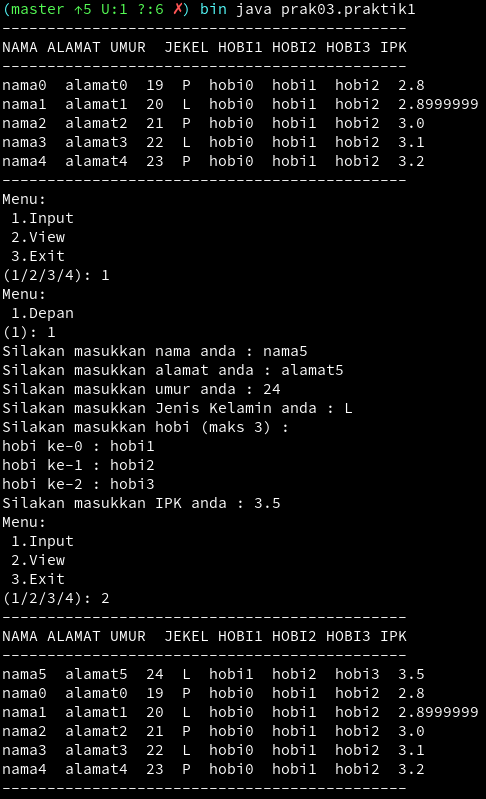
\includegraphics[scale=.7]{prak1.png} 
\end{center}

\subsubsection{Praktik 02}
\begin{lstlisting}
import java.util.Scanner;

class formatbiodata2 { // bagian deklarasi struktur record ---------------------------------
    String nama;
    String alamat;
    int umur;
    char jekel;
    String hobi[] = new String[3];
    float ipk;
}

class praktik2 {
    public static int N = 5;

    public static void isiData(formatbiodata2 biodataMahasiswa[]){
        float nilai = 0;
        for(int i = 0; i < N; i++){
            nilai = i / 10f;
            biodataMahasiswa[i].nama = "nama" + i;
            biodataMahasiswa[i].alamat = "alamat" + i;
            biodataMahasiswa[i].umur = 19 + i;
            if((i%2)!=0){
                biodataMahasiswa[i].jekel = 'L';
            }else{
                biodataMahasiswa[i].jekel = 'P';
            }
            for(int j = 0; j < 3; j++){
                biodataMahasiswa[i].hobi[j] = "hobi"+ j;
            }
            biodataMahasiswa[i].ipk = 2.8f + nilai;
        }
    }


    // --------------------------------------------------
    // --- Fungsi untuk Menambah Data Di Depan ---
    // --------------------------------------------------
    public static void tambahDataDiDepan(formatbiodata2 biodataMahasiswa[]) {
        // bagian membuat record sementara untuk menampung data baru-------------
        formatbiodata2 biodataMahasiswaBaru = new formatbiodata2();
        // bagian entri data baru ke penyimpan sementara-----------------------
        Scanner masukan = new Scanner(System.in);
        int bacaTombol = 0;
        System.out.print("Silakan masukkan nama anda : ");
        biodataMahasiswaBaru.nama = masukan.next();
        System.out.print("Silakan masukkan alamat anda : ");
        biodataMahasiswaBaru.alamat = masukan.next();
        System.out.print("Silakan masukkan umur anda : ");
        biodataMahasiswaBaru.umur = masukan.nextInt();
        System.out.print("Silakan masukkan Jenis Kelamin anda : ");
        try {
            bacaTombol = System.in.read();
        } catch (java.io.IOException e) {
        }
        biodataMahasiswaBaru.jekel = (char) bacaTombol;
        System.out.println("Silakan masukkan hobi (maks 3) : ");
        System.out.print("hobi ke-0 : ");
        biodataMahasiswaBaru.hobi[0] = masukan.next();
        System.out.print("hobi ke-1 : ");
        biodataMahasiswaBaru.hobi[1] = masukan.next();
        System.out.print("hobi ke-2 : ");
        biodataMahasiswaBaru.hobi[2] = masukan.next();
        System.out.print("Silakan masukkan IPK anda : ");
        biodataMahasiswaBaru.ipk = masukan.nextFloat();
        // bagian menggeser isi larik mulai dari Belakang s/d 0 selangkah ke bawah
        for (int i = N - 1; i >= 0; i--) {
            biodataMahasiswa[i + 1] = biodataMahasiswa[i];
        }
        // bagian memindahkan data baru ke larik ke-0-----------------------
        biodataMahasiswa[0] = biodataMahasiswaBaru;
        // memperbaharui banyaknya data (N), banyaknya data bertambah satu------
        N++;
    }

    // --------------------------------------------------
    // --- Fungsi untuk Menambah Data Di Tengah ---
    // --------------------------------------------------
    public static void tambahDataDiTengah(formatbiodata2 biodataMahasiswa[]) {
        // bagian membuat record sementara untuk menampung data baru-----------
        formatbiodata2 biodataMahasiswaBaru = new formatbiodata2();
        // bagian entri data baru ke penyimpan sementara-----------------------
        Scanner masukan = new Scanner(System.in);
        int bacaTombol = 0;
        System.out.print("Silakan masukkan nama anda : ");
        biodataMahasiswaBaru.nama = masukan.next();
        System.out.print("Silakan masukkan alamat anda : ");
        biodataMahasiswaBaru.alamat = masukan.next();
        System.out.print("Silakan masukkan umur anda : ");
        biodataMahasiswaBaru.umur = masukan.nextInt();
        System.out.print("Silakan masukkan Jenis Kelamin anda : ");
        try {
            bacaTombol = System.in.read();
        } catch (java.io.IOException e) {

        }
        biodataMahasiswaBaru.jekel = (char) bacaTombol;
        System.out.println("Silakan masukkan hobi (maks 3) : ");
        System.out.print("hobi ke-0 : ");
        biodataMahasiswaBaru.hobi[0] = masukan.next();
        System.out.print("hobi ke-1 : ");
        biodataMahasiswaBaru.hobi[1] = masukan.next();
        System.out.print("hobi ke-2 : ");
        biodataMahasiswaBaru.hobi[2] = masukan.next();
        System.out.print("Silakan masukkan IPK anda : ");
        biodataMahasiswaBaru.ipk = masukan.nextFloat();
        // bagian menentukan posisi target T ----------------------------------
        int T;
        System.out.print("Pada posisi ke berapa data akan dimasukkan ? : ");
        T = masukan.nextInt();
        T--;
        // bagian menggeser isi larik mulai dari Belakang s/d T selangkah ke belakang
        for (int i = N - 1; i >= T; i--) {
            biodataMahasiswa[i + 1] = biodataMahasiswa[i];
        }
        // bagian memindahkan data baru ke larik ke-T----------------------
        biodataMahasiswa[T] = biodataMahasiswaBaru;
        // memperbaharui banyaknya data (N), banyaknya data bertambah satu-------
        N++;
    }

    // --------------------------------------------------
    // --- Fungsi untuk menampilkan data ---
    // --------------------------------------------------
    public static void tampilkanData(formatbiodata2 biodataMahasiswa[]) {
        // bagian menampilkan isi struktur Larik --------------------------
        System.out.println("---------------------------------------------");
        System.out.println("NAMA ALAMAT UMUR  JEKEL HOBI1 HOBI2 HOBI3 IPK");
        System.out.println("---------------------------------------------");
        for (int i = 0; i <= N - 1; i++) {
            System.out.print(biodataMahasiswa[i].nama + "  ");
            System.out.print(biodataMahasiswa[i].alamat + "  ");
            System.out.print(biodataMahasiswa[i].umur + "  ");
            System.out.print(biodataMahasiswa[i].jekel + "  ");
            System.out.print(biodataMahasiswa[i].hobi[0] + "  ");
            System.out.print(biodataMahasiswa[i].hobi[1] + "  ");
            System.out.print(biodataMahasiswa[i].hobi[2] + "  ");
            System.out.println(biodataMahasiswa[i].ipk);
        }
        System.out.println("---------------------------------------------");
    }

    // --------------------------------------------------
    // --- Program Utama ---
    // --------------------------------------------------
    public static void main(String[] args) { // bagian deklarasi record berbasis LARIK -----------------------
        Scanner in = new Scanner(System.in);
        formatbiodata2 biodataMahasiswa[] = new formatbiodata2[10];
        biodataMahasiswa[0] = new formatbiodata2();
        biodataMahasiswa[1] = new formatbiodata2();
        biodataMahasiswa[2] = new formatbiodata2();
        biodataMahasiswa[3] = new formatbiodata2();
        biodataMahasiswa[4] = new formatbiodata2();
        isiData(biodataMahasiswa);
        tampilkanData(biodataMahasiswa);
        int jawab = 0;
        do {
            System.out.println("Menu:");
            System.out.printf(" 1.Input\n 2.View\n 3.Exit\n");
            System.out.print("(1/2/3/4): ");
            jawab = in.nextInt();
            switch (jawab) {
                case 1:
                    System.out.println("Menu:");
                    System.out.printf(" 1.Depan \n 2.Tengah\n");
                    System.out.print("(1/2/3): ");
                    int jawab2 = in.nextInt();
                    switch (jawab2) {
                        case 1:
                            tambahDataDiDepan(biodataMahasiswa);
                            break;
                        case 2:
                            tambahDataDiTengah(biodataMahasiswa);
                            break;
                    }
                    break;

                case 2:
                    tampilkanData(biodataMahasiswa);
                    break;

                default:
                    break;
            }
        } while (jawab != 3);
    }
}
\end{lstlisting}
Program tersebut merupakan program sebelumnya yang diberi fungsi untuk menambahkan data pada record, di bagian tengah
atau di bagian yang ditentukan oleh user.\\
Algoritma pada fungsi tambahDataDiTengah, adalah sebagai berikut.\\
Fungsi akan menciptakan  ruang kosong pada larik ke-T di mana T adalah posisi target kemudian memasukkan data baru pada
ruang kosong tersebut.Proses ini harus didahului dengan proses penggeseran data secara berturut-turut mulai dari data
terakhir sampai dengan data ke-T sebanyak satu langkah ke bawah sehingga akan menciptakan ruang kosong pada larik
ke-T, sementara data yang bergeser akan menempati larik ke-T+1 hingga larik terakhir+1. Setelah proses penggeseran data
selesai nilai N (banyaknya data) harus tambah dengan 1.\\
Jika program dijalankan maka akan seperti berikut:
\begin{center}
    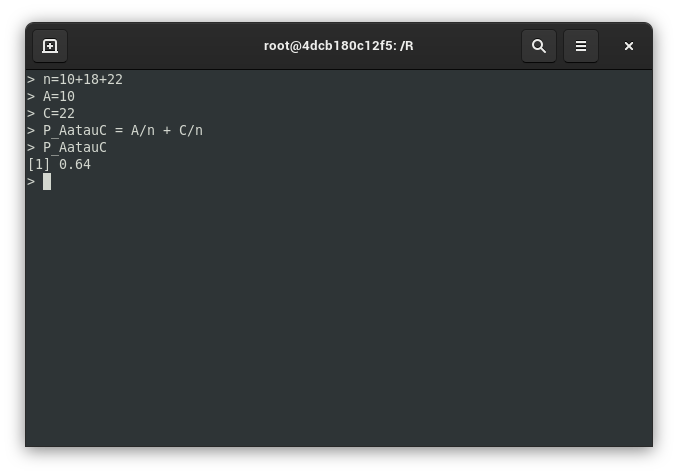
\includegraphics[scale=.7]{prak2.png} 
\end{center}

\subsubsection{Praktik 3}
\begin{lstlisting}
import java.util.Scanner;

class formatBiodata3 { // bagian deklarasi struktur record ---------------------------------
    String nama;
    String alamat;
    int umur;
    char jekel;
    String hobi[] = new String[3];
    float ipk;
}

class praktik3 {
    public static int N = 5;

    public static void isiData(formatBiodata3 biodataMahasiswa[]){
        float nilai = 0;
        for(int i = 0; i < N; i++){
            nilai = i / 10f;
            biodataMahasiswa[i].nama = "nama" + i;
            biodataMahasiswa[i].alamat = "alamat" + i;
            biodataMahasiswa[i].umur = 19 + i;
            if((i%2)!=0){
                biodataMahasiswa[i].jekel = 'L';
            }else{
                biodataMahasiswa[i].jekel = 'P';
            }
            for(int j = 0; j < 3; j++){
                biodataMahasiswa[i].hobi[j] = "hobi"+ j;
            }
            biodataMahasiswa[i].ipk = 2.8f + nilai;
        }
    }

    // --------------------------------------------------
    // --- Fungsi untuk Menambah Data Di Depan ---
    // --------------------------------------------------
    public static void tambahDataDiDepan(formatBiodata3 biodataMahasiswa[]) {
        // bagian membuat record sementara untuk menampung data baru-------------
        formatBiodata3 biodataMahasiswaBaru = new formatBiodata3();
        // bagian entri data baru ke penyimpan sementara-----------------------
        Scanner masukan = new Scanner(System.in);
        int bacaTombol = 0;
        System.out.print("Silakan masukkan nama anda : ");
        biodataMahasiswaBaru.nama = masukan.next();
        System.out.print("Silakan masukkan alamat anda : ");
        biodataMahasiswaBaru.alamat = masukan.next();
        System.out.print("Silakan masukkan umur anda : ");
        biodataMahasiswaBaru.umur = masukan.nextInt();
        System.out.print("Silakan masukkan Jenis Kelamin anda : ");
        try {
            bacaTombol = System.in.read();
        } catch (java.io.IOException e) {
        }
        biodataMahasiswaBaru.jekel = (char) bacaTombol;
        System.out.println("Silakan masukkan hobi (maks 3) : ");
        System.out.print("hobi ke-0 : ");
        biodataMahasiswaBaru.hobi[0] = masukan.next();
        System.out.print("hobi ke-1 : ");
        biodataMahasiswaBaru.hobi[1] = masukan.next();
        System.out.print("hobi ke-2 : ");
        biodataMahasiswaBaru.hobi[2] = masukan.next();
        System.out.print("Silakan masukkan IPK anda : ");
        biodataMahasiswaBaru.ipk = masukan.nextFloat();
        // bagian menggeser isi larik mulai dari Belakang s/d 0 selangkah ke bawah
        for (int i = N - 1; i >= 0; i--) {
            biodataMahasiswa[i + 1] = biodataMahasiswa[i];
        }
        // bagian memindahkan data baru ke larik ke-0-----------------------
        biodataMahasiswa[0] = biodataMahasiswaBaru;
        // memperbaharui banyaknya data (N), banyaknya data bertambah satu------
        N++;
    }

    // --------------------------------------------------
    // --- Fungsi untuk Menambah Data Di Tengah ---
    // --------------------------------------------------
    public static void tambahDataDiTengah(formatBiodata3 biodataMahasiswa[]) {
        // bagian membuat record sementara untuk menampung data baru-----------
        formatBiodata3 biodataMahasiswaBaru = new formatBiodata3();
        // bagian entri data baru ke penyimpan sementara-----------------------
        Scanner masukan = new Scanner(System.in);
        int bacaTombol = 0;
        System.out.print("Silakan masukkan nama anda : ");
        biodataMahasiswaBaru.nama = masukan.next();
        System.out.print("Silakan masukkan alamat anda : ");
        biodataMahasiswaBaru.alamat = masukan.next();
        System.out.print("Silakan masukkan umur anda : ");
        biodataMahasiswaBaru.umur = masukan.nextInt();
        System.out.print("Silakan masukkan Jenis Kelamin anda : ");
        try {
            bacaTombol = System.in.read();
        } catch (java.io.IOException e) {

        }
        biodataMahasiswaBaru.jekel = (char) bacaTombol;
        System.out.println("Silakan masukkan hobi (maks 3) : ");
        System.out.print("hobi ke-0 : ");
        biodataMahasiswaBaru.hobi[0] = masukan.next();
        System.out.print("hobi ke-1 : ");
        biodataMahasiswaBaru.hobi[1] = masukan.next();
        System.out.print("hobi ke-2 : ");
        biodataMahasiswaBaru.hobi[2] = masukan.next();
        System.out.print("Silakan masukkan IPK anda : ");
        biodataMahasiswaBaru.ipk = masukan.nextFloat();
        // bagian menentukan posisi target T ----------------------------------
        int T;
        System.out.print("Pada posisi ke berapa data akan dimasukkan ? : ");
        T = masukan.nextInt();
        T--;
        // bagian menggeser isi larik mulai dari Belakang s/d T selangkah ke belakang
        for (int i = N - 1; i >= T; i--) {
            biodataMahasiswa[i + 1] = biodataMahasiswa[i];
        }
        // bagian memindahkan data baru ke larik ke-T----------------------
        biodataMahasiswa[T] = biodataMahasiswaBaru;
        // memperbaharui banyaknya data (N), banyaknya data bertambah satu-------
        N++;
    }

    // --------------------------------------------------
    // --- Fungsi untuk Menambah Data Di Belakang ---
    // --------------------------------------------------
    public static void tambahDataDiBelakang(formatBiodata3 biodataMahasiswa[]) {
        // bagian membuat record sementara untuk menampung data baru-------------
        formatBiodata3 biodataMahasiswaBaru = new formatBiodata3();
        // bagian entri data baru ke penyimpan sementara-----------------------
        Scanner masukan = new Scanner(System.in);
        int bacaTombol = 0;
        System.out.print("Silakan masukkan nama anda : ");
        biodataMahasiswaBaru.nama = masukan.next();
        System.out.print("Silakan masukkan alamat anda : ");
        biodataMahasiswaBaru.alamat = masukan.next();
        System.out.print("Silakan masukkan umur anda : ");
        biodataMahasiswaBaru.umur = masukan.nextInt();
        System.out.print("Silakan masukkan Jenis Kelamin anda : ");
        try {
            bacaTombol = System.in.read();
        } catch (java.io.IOException e) {
        }
        biodataMahasiswaBaru.jekel = (char) bacaTombol;
        System.out.println("Silakan masukkan hobi (maks 3) : ");
        System.out.print("hobi ke-0 : ");
        biodataMahasiswaBaru.hobi[0] = masukan.next();
        System.out.print("hobi ke-1 : ");
        biodataMahasiswaBaru.hobi[1] = masukan.next();
        System.out.print("hobi ke-2 : ");
        biodataMahasiswaBaru.hobi[2] = masukan.next();
        System.out.print("Silakan masukkan IPK anda : ");
        biodataMahasiswaBaru.ipk = masukan.nextFloat();
        // bagian memindahkan data baru ke larik ke-N-----------------------
        biodataMahasiswa[N] = biodataMahasiswaBaru;
        // memperbaharui banyaknya data (N), banyaknya data bertambah satu----
        N++;
    }

    // --------------------------------------------------
    // --- Fungsi untuk menampilkan data ---
    // --------------------------------------------------
    public static void tampilkanData(formatBiodata3 biodataMahasiswa[]) {
        // bagian menampilkan isi struktur Larik --------------------------
        System.out.println("---------------------------------------------");
        System.out.println("NAMA ALAMAT UMUR  JEKEL HOBI1 HOBI2 HOBI3 IPK");
        System.out.println("---------------------------------------------");
        for (int i = 0; i <= N - 1; i++) {
            System.out.print(biodataMahasiswa[i].nama + "  ");
            System.out.print(biodataMahasiswa[i].alamat + "  ");
            System.out.print(biodataMahasiswa[i].umur + "  ");
            System.out.print(biodataMahasiswa[i].jekel + "  ");
            System.out.print(biodataMahasiswa[i].hobi[0] + "  ");
            System.out.print(biodataMahasiswa[i].hobi[1] + "  ");
            System.out.print(biodataMahasiswa[i].hobi[2] + "  ");
            System.out.println(biodataMahasiswa[i].ipk);
        }
        System.out.println("---------------------------------------------");
    }

    // --------------------------------------------------
    // --- Program Utama ---
    // --------------------------------------------------
    public static void main(String[] args) { // bagian deklarasi record berbasis LARIK -----------------------
        Scanner in = new Scanner(System.in);
        formatBiodata3 biodataMahasiswa[] = new formatBiodata3[10];
        biodataMahasiswa[0] = new formatBiodata3();
        biodataMahasiswa[1] = new formatBiodata3();
        biodataMahasiswa[2] = new formatBiodata3();
        biodataMahasiswa[3] = new formatBiodata3();
        biodataMahasiswa[4] = new formatBiodata3();
        isiData(biodataMahasiswa);
        tampilkanData(biodataMahasiswa);
        int jawab=0;
        do {
            System.out.println("Menu:");
            System.out.printf(" 1.Input\n 2.View\n 3.Exit\n");
            System.out.print("(1/2/3/4): ");
            jawab = in.nextInt();
            switch (jawab) {
                case 1:
                    System.out.println("Menu:");
                    System.out.printf(" 1.Depan \n 2.Tengah\n 3.Belakang\n");
                    System.out.print("(1/2/3): ");
                    int jawab2 = in.nextInt();
                    switch (jawab2) {
                        case 1:
                            tambahDataDiDepan(biodataMahasiswa);
                            break;
                        case 2:
                            tambahDataDiTengah(biodataMahasiswa);
                            break;
                        case 3:
                            tambahDataDiBelakang(biodataMahasiswa);
                            break;
                    }
                    break;

                case 2:
                    tampilkanData(biodataMahasiswa);
                    break;

                default:
                    break;
            }
        } while (jawab != 3);
    }
}
\end{lstlisting}
Pada praktik 3, program ditambah fungsi untuk menambahkan data pada record terakhir.\\
Algoritma pada fungsi tambahDataDiBelakang seperti berikut:\\
Fungsi tambahDataDiBelakang akan memasukkan data yang baru pada larik ke-N di mana N adalah posisi paling
akhir. Pada proses menambah data di belakang, program tidak perlu melakukan penggeseran data yang telah ada dalam larik
melainkan cukup dengan menaikkan nilai N nya saja (banyaknya data) dengan 1.

\subsubsection{Praktik 4}
\begin{lstlisting}
import java.util.Scanner;

class formatBiodata4 { // bagian deklarasi struktur record ---------------------------------
    String nama;
    String alamat;
    int umur;
    char jekel;
    String hobi[] = new String[3];
    float ipk;
}

class praktik4 {
    public static int N = 5;

    public static void isiData(formatBiodata4 biodataMahasiswa[]){
        float nilai = 0;
        for(int i = 0; i < N; i++){
            nilai = i / 10f;
            biodataMahasiswa[i].nama = "nama" + i;
            biodataMahasiswa[i].alamat = "alamat" + i;
            biodataMahasiswa[i].umur = 19 + i;
            if((i%2)!=0){
                biodataMahasiswa[i].jekel = 'L';
            }else{
                biodataMahasiswa[i].jekel = 'P';
            }
            for(int j = 0; j < 3; j++){
                biodataMahasiswa[i].hobi[j] = "hobi"+ j;
            }
            biodataMahasiswa[i].ipk = 2.8f + nilai;
        }
    }

    // --------------------------------------------------
    // --- Fungsi untuk Menambah Data Di Depan ---
    // --------------------------------------------------
    public static void tambahDataDiDepan(formatBiodata4 biodataMahasiswa[]) {
        // bagian membuat record sementara untuk menampung data baru-------------
        formatBiodata4 biodataMahasiswaBaru = new formatBiodata4();
        // bagian entri data baru ke penyimpan sementara-----------------------
        Scanner masukan = new Scanner(System.in);
        int bacaTombol = 0;
        System.out.print("Silakan masukkan nama anda : ");
        biodataMahasiswaBaru.nama = masukan.next();
        System.out.print("Silakan masukkan alamat anda : ");
        biodataMahasiswaBaru.alamat = masukan.next();
        System.out.print("Silakan masukkan umur anda : ");
        biodataMahasiswaBaru.umur = masukan.nextInt();
        System.out.print("Silakan masukkan Jenis Kelamin anda : ");
        try {
            bacaTombol = System.in.read();
        } catch (java.io.IOException e) {
        }
        biodataMahasiswaBaru.jekel = (char) bacaTombol;
        System.out.println("Silakan masukkan hobi (maks 3) : ");
        System.out.print("hobi ke-0 : ");
        biodataMahasiswaBaru.hobi[0] = masukan.next();
        System.out.print("hobi ke-1 : ");
        biodataMahasiswaBaru.hobi[1] = masukan.next();
        System.out.print("hobi ke-2 : ");
        biodataMahasiswaBaru.hobi[2] = masukan.next();
        System.out.print("Silakan masukkan IPK anda : ");
        biodataMahasiswaBaru.ipk = masukan.nextFloat();
        // bagian menggeser isi larik mulai dari Belakang s/d 0 selangkah ke bawah
        for (int i = N - 1; i >= 0; i--) {
            biodataMahasiswa[i + 1] = biodataMahasiswa[i];
        }
        // bagian memindahkan data baru ke larik ke-0-----------------------
        biodataMahasiswa[0] = biodataMahasiswaBaru;
        // memperbaharui banyaknya data (N), banyaknya data bertambah satu------
        N++;
    }

    // --------------------------------------------------
    // --- Fungsi untuk Menambah Data Di Tengah ---
    // --------------------------------------------------
    public static void tambahDataDiTengah(formatBiodata4 biodataMahasiswa[]) {
        // bagian membuat record sementara untuk menampung data baru-----------
        formatBiodata4 biodataMahasiswaBaru = new formatBiodata4();
        // bagian entri data baru ke penyimpan sementara-----------------------
        Scanner masukan = new Scanner(System.in);
        int bacaTombol = 0;
        System.out.print("Silakan masukkan nama anda : ");
        biodataMahasiswaBaru.nama = masukan.next();
        System.out.print("Silakan masukkan alamat anda : ");
        biodataMahasiswaBaru.alamat = masukan.next();
        System.out.print("Silakan masukkan umur anda : ");
        biodataMahasiswaBaru.umur = masukan.nextInt();
        System.out.print("Silakan masukkan Jenis Kelamin anda : ");
        try {
            bacaTombol = System.in.read();
        } catch (java.io.IOException e) {

        }
        biodataMahasiswaBaru.jekel = (char) bacaTombol;
        System.out.println("Silakan masukkan hobi (maks 3) : ");
        System.out.print("hobi ke-0 : ");
        biodataMahasiswaBaru.hobi[0] = masukan.next();
        System.out.print("hobi ke-1 : ");
        biodataMahasiswaBaru.hobi[1] = masukan.next();
        System.out.print("hobi ke-2 : ");
        biodataMahasiswaBaru.hobi[2] = masukan.next();
        System.out.print("Silakan masukkan IPK anda : ");
        biodataMahasiswaBaru.ipk = masukan.nextFloat();
        // bagian menentukan posisi target T ----------------------------------
        int T;
        System.out.print("Pada posisi ke berapa data akan dimasukkan ? : ");
        T = masukan.nextInt();
        T--;
        // bagian menggeser isi larik mulai dari Belakang s/d T selangkah ke belakang
        for (int i = N - 1; i >= T; i--) {
            biodataMahasiswa[i + 1] = biodataMahasiswa[i];
        }
        // bagian memindahkan data baru ke larik ke-T----------------------
        biodataMahasiswa[T] = biodataMahasiswaBaru;
        // memperbaharui banyaknya data (N), banyaknya data bertambah satu-------
        N++;
    }

    // --------------------------------------------------
    // --- Fungsi untuk Menambah Data Di Belakang ---
    // --------------------------------------------------
    public static void tambahDataDiBelakang(formatBiodata4 biodataMahasiswa[]) {
        // bagian membuat record sementara untuk menampung data baru-------------
        formatBiodata4 biodataMahasiswaBaru = new formatBiodata4();
        // bagian entri data baru ke penyimpan sementara-----------------------
        Scanner masukan = new Scanner(System.in);
        int bacaTombol = 0;
        System.out.print("Silakan masukkan nama anda : ");
        biodataMahasiswaBaru.nama = masukan.next();
        System.out.print("Silakan masukkan alamat anda : ");
        biodataMahasiswaBaru.alamat = masukan.next();
        System.out.print("Silakan masukkan umur anda : ");
        biodataMahasiswaBaru.umur = masukan.nextInt();
        System.out.print("Silakan masukkan Jenis Kelamin anda : ");
        try {
            bacaTombol = System.in.read();
        } catch (java.io.IOException e) {
        }
        biodataMahasiswaBaru.jekel = (char) bacaTombol;
        System.out.println("Silakan masukkan hobi (maks 3) : ");
        System.out.print("hobi ke-0 : ");
        biodataMahasiswaBaru.hobi[0] = masukan.next();
        System.out.print("hobi ke-1 : ");
        biodataMahasiswaBaru.hobi[1] = masukan.next();
        System.out.print("hobi ke-2 : ");
        biodataMahasiswaBaru.hobi[2] = masukan.next();
        System.out.print("Silakan masukkan IPK anda : ");
        biodataMahasiswaBaru.ipk = masukan.nextFloat();
        // bagian memindahkan data baru ke larik ke-N-----------------------
        biodataMahasiswa[N] = biodataMahasiswaBaru;
        // memperbaharui banyaknya data (N), banyaknya data bertambah satu----
        N++;
    }

    // --------------------------------------------------
    // --- Fungsi untuk Menghapus Data Di Depan ---
    // --------------------------------------------------
    public static void hapusDataDiDepan(formatBiodata4 biodataMahasiswa[]) {
        // bagian menggeser isi larik mulai dari 0 - Belakang selangkah ke depan
        for (int i = 0; i <= N - 2; i++) {
            biodataMahasiswa[i] = biodataMahasiswa[i + 1];
        }
        System.out.println("Proses menghapus data ke-0 selesai.");
        // memperbaharui banyaknya data (N), banyaknya data berkurang satu-------
        N--;
    }

    // --------------------------------------------------
    // --- Fungsi untuk Menghapus Data Di Tengah ---
    // --------------------------------------------------
    public static void hapusDataDiTengah(formatBiodata4 biodataMahasiswa[]) {
        // bagian menentukan posisi target T --------------------------------------
        Scanner masukan = new Scanner(System.in);
        int T;
        System.out.print("Tuliskan posisi data yang akan dibapus : ");
        T = masukan.nextInt();
        T--;
        // bagian menggeser isi larik mulai dari T - Belakang selangkah ke depan
        for (int i = T; i <= N - 2; i++) {
            biodataMahasiswa[i] = biodataMahasiswa[i + 1];
        }
        System.out.println("Proses menghapus data ke-" + T + " selesai.");
        // memperbaharui banyaknya data (N), banyaknya data berkurang satu-------
        N--;
    }

    // --------------------------------------------------
    // --- Fungsi untuk Menghapus Data Di Belakang ---
    // --------------------------------------------------
    public static void hapusDataDiBelakang(formatBiodata4 biodataMahasiswa[]) {
        System.out.println("Proses menghapus data paling akhir selesai.");
        // memperbaharui banyaknya data (N), banyaknya data berkurang satu-------
        N--;
    }

    // --------------------------------------------------
    // --- Fungsi untuk menampilkan data ---
    // --------------------------------------------------
    public static void tampilkanData(formatBiodata4 biodataMahasiswa[]) {
        // bagian menampilkan isi struktur Larik --------------------------
        System.out.println("---------------------------------------------");
        System.out.println("NAMA ALAMAT UMUR  JEKEL HOBI1 HOBI2 HOBI3 IPK");
        System.out.println("---------------------------------------------");
        for (int i = 0; i <= N - 1; i++) {
            System.out.print(biodataMahasiswa[i].nama + "  ");
            System.out.print(biodataMahasiswa[i].alamat + "  ");
            System.out.print(biodataMahasiswa[i].umur + "  ");
            System.out.print(biodataMahasiswa[i].jekel + "  ");
            System.out.print(biodataMahasiswa[i].hobi[0] + "  ");
            System.out.print(biodataMahasiswa[i].hobi[1] + "  ");
            System.out.print(biodataMahasiswa[i].hobi[2] + "  ");
            System.out.println(biodataMahasiswa[i].ipk);
        }
        System.out.println("---------------------------------------------");
    }

    // --------------------------------------------------
    // --- Program Utama ---
    // --------------------------------------------------
    public static void main(String[] args) { // bagian deklarasi record berbasis LARIK -----------------------
        Scanner in = new Scanner(System.in);
        formatBiodata4 biodataMahasiswa[] = new formatBiodata4[10];
        biodataMahasiswa[0] = new formatBiodata4();
        biodataMahasiswa[1] = new formatBiodata4();
        biodataMahasiswa[2] = new formatBiodata4();
        biodataMahasiswa[3] = new formatBiodata4();
        biodataMahasiswa[4] = new formatBiodata4();
        isiData(biodataMahasiswa);
        tampilkanData(biodataMahasiswa);
        int jawab=0;
        do {
            System.out.println("Menu:");
            System.out.printf(" 1.Input\n 2.View\n 3.Delete\n 4.Exit\n");
            System.out.print("(1/2/3/4): ");
            jawab = in.nextInt();
            switch (jawab) {
                case 1:
                    System.out.println("Menu:");
                    System.out.printf(" 1.Depan \n 2.Tengah\n 3.Belakang\n");
                    System.out.print("(1/2/3): ");
                    int jawab2 = in.nextInt();
                    switch (jawab2) {
                        case 1:
                            tambahDataDiDepan(biodataMahasiswa);
                            break;
                        case 2:
                            tambahDataDiTengah(biodataMahasiswa);
                            break;
                        case 3:
                            tambahDataDiBelakang(biodataMahasiswa);
                            break;
                    }
                    break;

                case 2:
                    tampilkanData(biodataMahasiswa);
                    break;

                case 3:
                    System.out.println("Menu:");
                    System.out.printf(" 1.Depan \n 2.Tengah\n 3.Belakang\n");
                    System.out.print("(1/2/3): ");
                    jawab = in.nextInt();
                    switch (jawab) {
                        case 1:
                            hapusDataDiDepan(biodataMahasiswa);
                            break;
                        case 2:
                            hapusDataDiTengah(biodataMahasiswa);
                            break;
                        case 3:
                            hapusDataDiBelakang(biodataMahasiswa);
                            break;
                    }
                    break;

                default:
                    break;
            }
        } while (jawab != 4);
    }
}
\end{lstlisting}
Pada praktik 4 ini, adalah menambah fungsi untuk menghapus data, baiki di depan, di tengah, maupun di belakang.\\
terdapat tiga fungsi menghapus yang ditambahkan pada program pada praktik ini.\\
Fungsi hapusDataDiDepan memiliki algoritma seperti berikut:\\
Menghapus data di bagian depan dilakukan dengan cara menimpa larik paling depan (larik ke-0) dengan larik ke-1,
dilanjutkan dengan menimpa larik ke-1 dengan larik ke-2, ke-2 dengan ke-3, dan seterusnya. Proses ini sama dengan
melakukan penggeseran secara berturut-turut data dimulai ke-0 sampai dengan data terakhir sebanyak satu langkah ke
depan. Setelah proses penggeseran selesai nilai N (banyaknya data)akan dikurangi 1.\\
Fungsi hapusDataDiTengah memiliki algoritma seperti berikut:\\
Menghapusdata di bagian tengah dilakukan dengan menentukan posisi target data yang ingin dihapus (T). Kemudian data yang
akan dihapus pada larik ke-T ditimpa dengan larik ke-T+1, dilanjutkan dengan menimpa larik ke-T+1 dengan larik ke-T+2,
larik ke-T+2 dengan ke-T+3, dan seterusnya. Proses ini sama dengan menggeser data mulai dari data ke-T+1 sampai dengan
data terakhir sebanyak satu langkah ke atas.\\
Sdangkan fungsi hapusDataDiBelakang algoritmanya seperti berikut:\\
Menghapus data di bagian belakang dilakukan tidak perlu ada penggeseran data. Proses menghapus data di bagian belakang
hanya dilakukan dengan memotong data terakhir dengan cara mengurangkan N dengan 1 (N--).

\newpage
\subsection{Latihan}
\begin{lstlisting}
import java.util.Scanner;

class formatBiodataL { // bagian deklarasi struktur record ---------------------------------
    String nama;
    String alamat;
    int umur;
    char jekel;
    String hobi[] = new String[3];
    float ipk;
}

class Latihan01 {
    public static int N = 5;

    public static void isiData(formatBiodataL biodataMahasiswa[]) {
        float nilai = 0;
        for (int i = 0; i < N; i++) {
            nilai = i / 10f;
            biodataMahasiswa[i].nama = "nama" + i;
            biodataMahasiswa[i].alamat = "alamat" + i;
            biodataMahasiswa[i].umur = 19 + i;
            if ((i % 2) != 0) {
                biodataMahasiswa[i].jekel = 'L';
            } else {
                biodataMahasiswa[i].jekel = 'P';
            }
            for (int j = 0; j < 3; j++) {
                biodataMahasiswa[i].hobi[j] = "hobi" + j;
            }
            biodataMahasiswa[i].ipk = 2.8f + nilai;
        }
    }

    // --------------------------------------------------
    // --- Fungsi untuk mengentri data ke dalam Larik ---
    // --------------------------------------------------
    public static void ngentriData(formatBiodataL biodataMahasiswa[]) {
        // bagian entri data ke dalam struktur larik ----------------
        Scanner masukan = new Scanner(System.in);
        int bacaTombol = 0;
        for (int i = 0; i <= N - 1; i++) {
            System.out.print("Silakan masukkan nama anda : ");
            biodataMahasiswa[i].nama = masukan.next();
            System.out.print("Silakan masukkan alamat anda : ");
            biodataMahasiswa[i].alamat = masukan.next();
            System.out.print("Silakan masukkan umur anda : ");
            biodataMahasiswa[i].umur = masukan.nextInt();
            System.out.print("Silakan masukkan Jenis Kelamin anda : ");
            try {
                bacaTombol = System.in.read();
            } catch (java.io.IOException e) {
            }
            biodataMahasiswa[i].jekel = (char) bacaTombol;
            System.out.println("Silakan masukkan hobi (maks 3) : ");
            System.out.print("hobi ke-0 : ");
            biodataMahasiswa[i].hobi[0] = masukan.next();
            System.out.print("hobi ke-1 : ");
            biodataMahasiswa[i].hobi[1] = masukan.next();
            System.out.print("hobi ke-2 : ");
            biodataMahasiswa[i].hobi[2] = masukan.next();
            System.out.print("Silakan masukkan IPK anda : ");
            biodataMahasiswa[i].ipk = masukan.nextFloat();
            System.out.println();
        }
    }

    // --------------------------------------------------
    // --- Fungsi untuk Menambah Data Di Depan ---
    // --------------------------------------------------
    public static void tambahDataDiDepan(formatBiodataL biodataMahasiswa[]) {
        // bagian membuat record sementara untuk menampung data baru-------------
        formatBiodataL biodataMahasiswaBaru = new formatBiodataL();
        // bagian entri data baru ke penyimpan sementara-----------------------
        Scanner masukan = new Scanner(System.in);
        int bacaTombol = 0;
        System.out.print("Silakan masukkan nama anda : ");
        biodataMahasiswaBaru.nama = masukan.next();
        System.out.print("Silakan masukkan alamat anda : ");
        biodataMahasiswaBaru.alamat = masukan.next();
        System.out.print("Silakan masukkan umur anda : ");
        biodataMahasiswaBaru.umur = masukan.nextInt();
        System.out.print("Silakan masukkan Jenis Kelamin anda : ");
        try {
            bacaTombol = System.in.read();
        } catch (java.io.IOException e) {
        }
        biodataMahasiswaBaru.jekel = (char) bacaTombol;
        System.out.println("Silakan masukkan hobi (maks 3) : ");
        System.out.print("hobi ke-0 : ");
        biodataMahasiswaBaru.hobi[0] = masukan.next();
        System.out.print("hobi ke-1 : ");
        biodataMahasiswaBaru.hobi[1] = masukan.next();
        System.out.print("hobi ke-2 : ");
        biodataMahasiswaBaru.hobi[2] = masukan.next();
        System.out.print("Silakan masukkan IPK anda : ");
        biodataMahasiswaBaru.ipk = masukan.nextFloat();
        // bagian menggeser isi larik mulai dari Belakang s/d 0 selangkah ke bawah
        for (int i = N - 1; i >= 0; i--) {
            biodataMahasiswa[i + 1] = biodataMahasiswa[i];
        }
        // bagian memindahkan data baru ke larik ke-0-----------------------
        biodataMahasiswa[0] = biodataMahasiswaBaru;
        // memperbaharui banyaknya data (N), banyaknya data bertambah satu------
        N++;
    }

    // --------------------------------------------------
    // --- Fungsi untuk Menambah Data Di Tengah ---
    // --------------------------------------------------
    public static void tambahDataDiTengah(formatBiodataL biodataMahasiswa[]) {
        // bagian membuat record sementara untuk menampung data baru-----------
        formatBiodataL biodataMahasiswaBaru = new formatBiodataL();
        // bagian entri data baru ke penyimpan sementara-----------------------
        Scanner masukan = new Scanner(System.in);
        int bacaTombol = 0;
        System.out.print("Silakan masukkan nama anda : ");
        biodataMahasiswaBaru.nama = masukan.next();
        System.out.print("Silakan masukkan alamat anda : ");
        biodataMahasiswaBaru.alamat = masukan.next();
        System.out.print("Silakan masukkan umur anda : ");
        biodataMahasiswaBaru.umur = masukan.nextInt();
        System.out.print("Silakan masukkan Jenis Kelamin anda : ");
        try {
            bacaTombol = System.in.read();
        } catch (java.io.IOException e) {

        }
        biodataMahasiswaBaru.jekel = (char) bacaTombol;
        System.out.println("Silakan masukkan hobi (maks 3) : ");
        System.out.print("hobi ke-0 : ");
        biodataMahasiswaBaru.hobi[0] = masukan.next();
        System.out.print("hobi ke-1 : ");
        biodataMahasiswaBaru.hobi[1] = masukan.next();
        System.out.print("hobi ke-2 : ");
        biodataMahasiswaBaru.hobi[2] = masukan.next();
        System.out.print("Silakan masukkan IPK anda : ");
        biodataMahasiswaBaru.ipk = masukan.nextFloat();
        // bagian menentukan posisi target T ----------------------------------
        int T;
        System.out.print("Pada posisi ke berapa data akan dimasukkan ? : ");
        T = masukan.nextInt();
        T--;
        // bagian menggeser isi larik mulai dari Belakang s/d T selangkah ke belakang
        for (int i = N - 1; i >= T; i--) {
            biodataMahasiswa[i + 1] = biodataMahasiswa[i];
        }
        // bagian memindahkan data baru ke larik ke-T----------------------
        biodataMahasiswa[T] = biodataMahasiswaBaru;
        // memperbaharui banyaknya data (N), banyaknya data bertambah satu-------
        N++;
    }

    // --------------------------------------------------
    // --- Fungsi untuk Menambah Data Di Belakang ---
    // --------------------------------------------------
    public static void tambahDataDiBelakang(formatBiodataL biodataMahasiswa[]) {
        // bagian membuat record sementara untuk menampung data baru-------------
        formatBiodataL biodataMahasiswaBaru = new formatBiodataL();
        // bagian entri data baru ke penyimpan sementara-----------------------
        Scanner masukan = new Scanner(System.in);
        int bacaTombol = 0;
        System.out.print("Silakan masukkan nama anda : ");
        biodataMahasiswaBaru.nama = masukan.next();
        System.out.print("Silakan masukkan alamat anda : ");
        biodataMahasiswaBaru.alamat = masukan.next();
        System.out.print("Silakan masukkan umur anda : ");
        biodataMahasiswaBaru.umur = masukan.nextInt();
        System.out.print("Silakan masukkan Jenis Kelamin anda : ");
        try {
            bacaTombol = System.in.read();
        } catch (java.io.IOException e) {
        }
        biodataMahasiswaBaru.jekel = (char) bacaTombol;
        System.out.println("Silakan masukkan hobi (maks 3) : ");
        System.out.print("hobi ke-0 : ");
        biodataMahasiswaBaru.hobi[0] = masukan.next();
        System.out.print("hobi ke-1 : ");
        biodataMahasiswaBaru.hobi[1] = masukan.next();
        System.out.print("hobi ke-2 : ");
        biodataMahasiswaBaru.hobi[2] = masukan.next();
        System.out.print("Silakan masukkan IPK anda : ");
        biodataMahasiswaBaru.ipk = masukan.nextFloat();
        // bagian memindahkan data baru ke larik ke-N-----------------------
        biodataMahasiswa[N] = biodataMahasiswaBaru;
        // memperbaharui banyaknya data (N), banyaknya data bertambah satu----
        N++;
    }

    // --------------------------------------------------
    // --- Fungsi untuk Menghapus Data Di Depan ---
    // --------------------------------------------------
    public static void hapusDataDiDepan(formatBiodataL biodataMahasiswa[]) {
        // bagian menggeser isi larik mulai dari 0 - Belakang selangkah ke depan
        for (int i = 0; i <= N - 2; i++) {
            biodataMahasiswa[i] = biodataMahasiswa[i + 1];
        }
        System.out.println("Proses menghapus data ke-0 selesai.");
        // memperbaharui banyaknya data (N), banyaknya data berkurang satu-------
        N--;
    }

    // --------------------------------------------------
    // --- Fungsi untuk Menghapus Data Di Tengah ---
    // --------------------------------------------------
    public static void hapusDataDiTengah(formatBiodataL biodataMahasiswa[]) {
        // bagian menentukan posisi target T --------------------------------------
        Scanner masukan = new Scanner(System.in);
        int T;
        System.out.print("Tuliskan posisi data yang akan dibapus : ");
        T = masukan.nextInt();
        // bagian menggeser isi larik mulai dari T - Belakang selangkah ke depan
        for (int i = T; i <= N - 2; i++) {
            biodataMahasiswa[i] = biodataMahasiswa[i + 1];
        }
        System.out.println("Proses menghapus data ke-" + T + " selesai.");
        // memperbaharui banyaknya data (N), banyaknya data berkurang satu-------
        N--;
    }

    // --------------------------------------------------
    // --- Fungsi untuk Menghapus Data Di Belakang ---
    // --------------------------------------------------
    public static void hapusDataDiBelakang(formatBiodataL biodataMahasiswa[]) {
        System.out.println("Proses menghapus data paling akhir selesai.");
        // memperbaharui banyaknya data (N), banyaknya data berkurang satu-------
        N--;
    }

    public static void tukarData(formatBiodataL biodataMahasiswa[]) {
        Scanner masukan = new Scanner(System.in);
        formatBiodataL tmpBiodata = new formatBiodataL();
        System.out.print("Tukar baris ini: ");
        int T = masukan.nextInt();
        System.out.print("Dengan baris ini: ");
        int T2 = masukan.nextInt();
        T--;
        T2--;
        tmpBiodata = biodataMahasiswa[T];
        biodataMahasiswa[T] = biodataMahasiswa[T2];
        biodataMahasiswa[T2] = tmpBiodata;
    }

    // --------------------------------------------------
    // --- Fungsi untuk menampilkan data ---
    // --------------------------------------------------
    public static void tampilkanData(formatBiodataL biodataMahasiswa[]) {
        // bagian menampilkan isi struktur Larik --------------------------
        System.out.println("---------------------------------------------");
        System.out.println("NAMA ALAMAT UMUR  JEKEL HOBI1 HOBI2 HOBI3 IPK");
        System.out.println("---------------------------------------------");
        for (int i = 0; i <= N - 1; i++) {
            System.out.print(biodataMahasiswa[i].nama + "  ");
            System.out.print(biodataMahasiswa[i].alamat + "  ");
            System.out.print(biodataMahasiswa[i].umur + "  ");
            System.out.print(biodataMahasiswa[i].jekel + "  ");
            System.out.print(biodataMahasiswa[i].hobi[0] + "  ");
            System.out.print(biodataMahasiswa[i].hobi[1] + "  ");
            System.out.print(biodataMahasiswa[i].hobi[2] + "  ");
            System.out.println(biodataMahasiswa[i].ipk);
        }
        System.out.println("---------------------------------------------");
    }

    // --------------------------------------------------
    // --- Program Utama ---
    // --------------------------------------------------
    public static void main(String[] args) { // bagian deklarasi record berbasis LARIK -----------------------
        Scanner in = new Scanner(System.in);
        formatBiodataL biodataMahasiswa[] = new formatBiodataL[10];
        biodataMahasiswa[0] = new formatBiodataL();
        biodataMahasiswa[1] = new formatBiodataL();
        biodataMahasiswa[2] = new formatBiodataL();
        biodataMahasiswa[3] = new formatBiodataL();
        biodataMahasiswa[4] = new formatBiodataL();
        isiData(biodataMahasiswa);
        tampilkanData(biodataMahasiswa);
        int jawab = 0;
        do {
            System.out.println("Menu:");
            System.out.printf(" 1.Input\n 2.View\n 3.Delete\n 4.Swap\n 5.Exit\n");
            System.out.print("(1/2/3/4): ");
            jawab = in.nextInt();
            switch (jawab) {
                case 1:
                    System.out.println("Menu:");
                    System.out.printf(" 1.Depan \n 2.Tengah\n 3.Belakang\n");
                    System.out.print("(1/2/3): ");
                    int jawab2 = in.nextInt();
                    switch (jawab2) {
                        case 1:
                            tambahDataDiDepan(biodataMahasiswa);
                            break;
                        case 2:
                            tambahDataDiTengah(biodataMahasiswa);
                            break;
                        case 3:
                            tambahDataDiBelakang(biodataMahasiswa);
                            break;
                    }
                    break;

                case 2:
                    tampilkanData(biodataMahasiswa);
                    break;

                case 3:
                    System.out.println("Menu:");
                    System.out.printf(" 1.Depan \n 2.Tengah\n 3.Belakang\n");
                    System.out.print("(1/2/3): ");
                    jawab = in.nextInt();
                    switch (jawab) {
                        case 1:
                            hapusDataDiDepan(biodataMahasiswa);
                            break;
                        case 2:
                            hapusDataDiTengah(biodataMahasiswa);
                            break;
                        case 3:
                            hapusDataDiBelakang(biodataMahasiswa);
                            break;
                    }
                    break;

                case 4:
                    tukarData(biodataMahasiswa);
                    break;

                default:
                    break;
            }
        } while (jawab != 5);
    }
\end{lstlisting}
Pada program latihan ini, program ditambah fungsi untuk menukar data.\\
Fungsi tukarData pada program tersebut memiliki algoritma penukaran data,
dengan cara menyimpan terlebih dahulu record T, ke dalam variabel untuk
menyimpan nilai sementara, lalu record T2, nilainya dipindah ke record T.
Kemudian nilai yang ada di variabel sementara tadi, dipindah ke record T2.
\begin{center}
    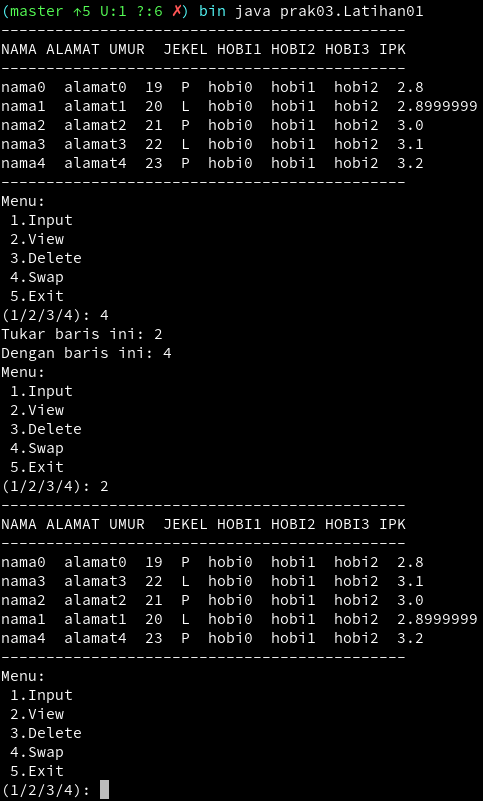
\includegraphics[scale=.7]{lat.png} 
\end{center}

\newpage
\subsection{Tugas}
\begin{lstlisting}
import java.util.Scanner;

class formatBiodataT { // bagian deklarasi struktur record ---------------------------------
    String nama;
    String alamat;
    int umur;
    char jekel;
    String hobi[] = new String[3];
    float ipk;
}

class Tugas01 {
    public static int N = 5;
    public static void isiData(formatBiodataT biodataMahasiswa[]){
        float nilai = 0;
        for(int i = 0; i < N; i++){
            nilai = i / 10f;
            biodataMahasiswa[i].nama = "nama" + i;
            biodataMahasiswa[i].alamat = "alamat" + i;
            biodataMahasiswa[i].umur = 19 + i;
            if((i%2)!=0){
                biodataMahasiswa[i].jekel = 'L';
            }else{
                biodataMahasiswa[i].jekel = 'P';
            }
            for(int j = 0; j < 3; j++){
                biodataMahasiswa[i].hobi[j] = "hobi"+ j;
            }
            biodataMahasiswa[i].ipk = 2.8f + nilai;
        }
    }

    // --------------------------------------------------
    // --- Fungsi untuk mengentri data ke dalam Larik ---
    // --------------------------------------------------
    public static void ngentriData(formatBiodataT biodataMahasiswa[]) {
        // bagian entri data ke dalam struktur larik ----------------
        Scanner masukan = new Scanner(System.in);
        int bacaTombol = 0;
        for (int i = 0; i <= N - 1; i++) {
            System.out.print("Silakan masukkan nama anda : ");
            biodataMahasiswa[i].nama = masukan.next();
            System.out.print("Silakan masukkan alamat anda : ");
            biodataMahasiswa[i].alamat = masukan.next();
            System.out.print("Silakan masukkan umur anda : ");
            biodataMahasiswa[i].umur = masukan.nextInt();
            System.out.print("Silakan masukkan Jenis Kelamin anda : ");
            try {
                bacaTombol = System.in.read();
            } catch (java.io.IOException e) {
            }
            biodataMahasiswa[i].jekel = (char) bacaTombol;
            System.out.println("Silakan masukkan hobi (maks 3) : ");
            System.out.print("hobi ke-0 : ");
            biodataMahasiswa[i].hobi[0] = masukan.next();
            System.out.print("hobi ke-1 : ");
            biodataMahasiswa[i].hobi[1] = masukan.next();
            System.out.print("hobi ke-2 : ");
            biodataMahasiswa[i].hobi[2] = masukan.next();
            System.out.print("Silakan masukkan IPK anda : ");
            biodataMahasiswa[i].ipk = masukan.nextFloat();
            System.out.println();
        }
    }

    // --------------------------------------------------
    // --- Fungsi untuk Menambah Data Di Depan ---
    // --------------------------------------------------
    public static void tambahDataDiDepan(formatBiodataT biodataMahasiswa[]) {
        // bagian membuat record sementara untuk menampung data baru-------------
        formatBiodataT biodataMahasiswaBaru = new formatBiodataT();
        // bagian entri data baru ke penyimpan sementara-----------------------
        Scanner masukan = new Scanner(System.in);
        int bacaTombol = 0;
        System.out.print("Silakan masukkan nama anda : ");
        biodataMahasiswaBaru.nama = masukan.next();
        System.out.print("Silakan masukkan alamat anda : ");
        biodataMahasiswaBaru.alamat = masukan.next();
        System.out.print("Silakan masukkan umur anda : ");
        biodataMahasiswaBaru.umur = masukan.nextInt();
        System.out.print("Silakan masukkan Jenis Kelamin anda : ");
        try {
            bacaTombol = System.in.read();
        } catch (java.io.IOException e) {
        }
        biodataMahasiswaBaru.jekel = (char) bacaTombol;
        System.out.println("Silakan masukkan hobi (maks 3) : ");
        System.out.print("hobi ke-0 : ");
        biodataMahasiswaBaru.hobi[0] = masukan.next();
        System.out.print("hobi ke-1 : ");
        biodataMahasiswaBaru.hobi[1] = masukan.next();
        System.out.print("hobi ke-2 : ");
        biodataMahasiswaBaru.hobi[2] = masukan.next();
        System.out.print("Silakan masukkan IPK anda : ");
        biodataMahasiswaBaru.ipk = masukan.nextFloat();
        // bagian menggeser isi larik mulai dari Belakang s/d 0 selangkah ke bawah
        for (int i = N - 1; i >= 0; i--) {
            biodataMahasiswa[i + 1] = biodataMahasiswa[i];
        }
        // bagian memindahkan data baru ke larik ke-0-----------------------
        biodataMahasiswa[0] = biodataMahasiswaBaru;
        // memperbaharui banyaknya data (N), banyaknya data bertambah satu------
        N++;
    }

    // --------------------------------------------------
    // --- Fungsi untuk Menambah Data Di Tengah ---
    // --------------------------------------------------
    public static void tambahDataDiTengah(formatBiodataT biodataMahasiswa[]) {
        // bagian membuat record sementara untuk menampung data baru-----------
        formatBiodataT biodataMahasiswaBaru = new formatBiodataT();
        // bagian entri data baru ke penyimpan sementara-----------------------
        Scanner masukan = new Scanner(System.in);
        int bacaTombol = 0;
        System.out.print("Silakan masukkan nama anda : ");
        biodataMahasiswaBaru.nama = masukan.next();
        System.out.print("Silakan masukkan alamat anda : ");
        biodataMahasiswaBaru.alamat = masukan.next();
        System.out.print("Silakan masukkan umur anda : ");
        biodataMahasiswaBaru.umur = masukan.nextInt();
        System.out.print("Silakan masukkan Jenis Kelamin anda : ");
        try {
            bacaTombol = System.in.read();
        } catch (java.io.IOException e) {

        }
        biodataMahasiswaBaru.jekel = (char) bacaTombol;
        System.out.println("Silakan masukkan hobi (maks 3) : ");
        System.out.print("hobi ke-0 : ");
        biodataMahasiswaBaru.hobi[0] = masukan.next();
        System.out.print("hobi ke-1 : ");
        biodataMahasiswaBaru.hobi[1] = masukan.next();
        System.out.print("hobi ke-2 : ");
        biodataMahasiswaBaru.hobi[2] = masukan.next();
        System.out.print("Silakan masukkan IPK anda : ");
        biodataMahasiswaBaru.ipk = masukan.nextFloat();
        // bagian menentukan posisi target T ----------------------------------
        int T;
        System.out.print("Pada posisi ke berapa data akan dimasukkan ? : ");
        T = masukan.nextInt();
        T--;
        // bagian menggeser isi larik mulai dari Belakang s/d T selangkah ke belakang
        for (int i = N - 1; i >= T; i--) {
            biodataMahasiswa[i + 1] = biodataMahasiswa[i];
        }
        // bagian memindahkan data baru ke larik ke-T----------------------
        biodataMahasiswa[T] = biodataMahasiswaBaru;
        // memperbaharui banyaknya data (N), banyaknya data bertambah satu-------
        N++;
    }

    // --------------------------------------------------
    // --- Fungsi untuk Menambah Data Di Belakang ---
    // --------------------------------------------------
    public static void tambahDataDiBelakang(formatBiodataT biodataMahasiswa[]) {
        // bagian membuat record sementara untuk menampung data baru-------------
        formatBiodataT biodataMahasiswaBaru = new formatBiodataT();
        // bagian entri data baru ke penyimpan sementara-----------------------
        Scanner masukan = new Scanner(System.in);
        int bacaTombol = 0;
        System.out.print("Silakan masukkan nama anda : ");
        biodataMahasiswaBaru.nama = masukan.next();
        System.out.print("Silakan masukkan alamat anda : ");
        biodataMahasiswaBaru.alamat = masukan.next();
        System.out.print("Silakan masukkan umur anda : ");
        biodataMahasiswaBaru.umur = masukan.nextInt();
        System.out.print("Silakan masukkan Jenis Kelamin anda : ");
        try {
            bacaTombol = System.in.read();
        } catch (java.io.IOException e) {
        }
        biodataMahasiswaBaru.jekel = (char) bacaTombol;
        System.out.println("Silakan masukkan hobi (maks 3) : ");
        System.out.print("hobi ke-0 : ");
        biodataMahasiswaBaru.hobi[0] = masukan.next();
        System.out.print("hobi ke-1 : ");
        biodataMahasiswaBaru.hobi[1] = masukan.next();
        System.out.print("hobi ke-2 : ");
        biodataMahasiswaBaru.hobi[2] = masukan.next();
        System.out.print("Silakan masukkan IPK anda : ");
        biodataMahasiswaBaru.ipk = masukan.nextFloat();
        // bagian memindahkan data baru ke larik ke-N-----------------------
        biodataMahasiswa[N] = biodataMahasiswaBaru;
        // memperbaharui banyaknya data (N), banyaknya data bertambah satu----
        N++;
    }

    // --------------------------------------------------
    // --- Fungsi untuk Menghapus Data Di Depan ---
    // --------------------------------------------------
    public static void hapusDataDiDepan(formatBiodataT biodataMahasiswa[]) {
        // bagian menggeser isi larik mulai dari 0 - Belakang selangkah ke depan
        for (int i = 0; i <= N - 2; i++) {
            biodataMahasiswa[i] = biodataMahasiswa[i + 1];
        }
        System.out.println("Proses menghapus data ke-0 selesai.");
        // memperbaharui banyaknya data (N), banyaknya data berkurang satu-------
        N--;
    }

    // --------------------------------------------------
    // --- Fungsi untuk Menghapus Data Di Tengah ---
    // --------------------------------------------------
    public static void hapusDataDiTengah(formatBiodataT biodataMahasiswa[]) {
        // bagian menentukan posisi target T --------------------------------------
        Scanner masukan = new Scanner(System.in);
        int T;
        System.out.print("Tuliskan posisi data yang akan dibapus : ");
        T = masukan.nextInt();
        T--;
        // bagian menggeser isi larik mulai dari T - Belakang selangkah ke depan
        for (int i = T; i <= N - 2; i++) {
            biodataMahasiswa[i] = biodataMahasiswa[i + 1];
        }
        System.out.println("Proses menghapus data ke-" + T + " selesai.");
        // memperbaharui banyaknya data (N), banyaknya data berkurang satu-------
        N--;
    }

    // --------------------------------------------------
    // --- Fungsi untuk Menghapus Data Di Belakang ---
    // --------------------------------------------------
    public static void hapusDataDiBelakang(formatBiodataT biodataMahasiswa[]) {
        System.out.println("Proses menghapus data paling akhir selesai.");
        // memperbaharui banyaknya data (N), banyaknya data berkurang satu-------
        N--;
    }

    public static void tukarData(formatBiodataT biodataMahasiswa[]) {
        Scanner masukan = new Scanner(System.in);
        formatBiodataT tmpBiodata = new formatBiodataT();
        System.out.print("Tukar baris ini: ");
        int T = masukan.nextInt();
        System.out.print("Dengan baris ini: ");
        int T2 = masukan.nextInt();
        T--;
        T2--;
        tmpBiodata = biodataMahasiswa[T];
        biodataMahasiswa[T] = biodataMahasiswa[T2];
        biodataMahasiswa[T2] = tmpBiodata;
    }

    public static void editData(formatBiodataT biodataMahasiswa[]) {
        Scanner masukan = new Scanner(System.in);
        formatBiodataT tmpBiodata = new formatBiodataT();
        System.out.print("Baris data yang dirubah: ");
        int T = masukan.nextInt();
        T--;
        int bacaTombol = 0;
        System.out.print("Silakan masukkan nama anda : ");
        tmpBiodata.nama = masukan.next();
        System.out.print("Silakan masukkan alamat anda : ");
        tmpBiodata.alamat = masukan.next();
        System.out.print("Silakan masukkan umur anda : ");
        tmpBiodata.umur = masukan.nextInt();
        System.out.print("Silakan masukkan Jenis Kelamin anda : ");
        try {
            bacaTombol = System.in.read();
        } catch (java.io.IOException e) {
        }
        tmpBiodata.jekel = (char) bacaTombol;
        System.out.println("Silakan masukkan hobi (maks 3) : ");
        System.out.print("hobi ke-0 : ");
        tmpBiodata.hobi[0] = masukan.next();
        System.out.print("hobi ke-1 : ");
        tmpBiodata.hobi[1] = masukan.next();
        System.out.print("hobi ke-2 : ");
        tmpBiodata.hobi[2] = masukan.next();
        System.out.print("Silakan masukkan IPK anda : ");
        tmpBiodata.ipk = masukan.nextFloat();
        biodataMahasiswa[T]=tmpBiodata;
    }

    // --------------------------------------------------
    // --- Fungsi untuk menampilkan data ---
    // --------------------------------------------------
    public static void tampilkanData(formatBiodataT biodataMahasiswa[]) {
        // bagian menampilkan isi struktur Larik --------------------------
        System.out.println("---------------------------------------------");
        System.out.println("NAMA ALAMAT UMUR  JEKEL HOBI1 HOBI2 HOBI3 IPK");
        System.out.println("---------------------------------------------");
        for (int i = 0; i <= N - 1; i++) {
            System.out.print(biodataMahasiswa[i].nama + "  ");
            System.out.print(biodataMahasiswa[i].alamat + "  ");
            System.out.print(biodataMahasiswa[i].umur + "  ");
            System.out.print(biodataMahasiswa[i].jekel + "  ");
            System.out.print(biodataMahasiswa[i].hobi[0] + "  ");
            System.out.print(biodataMahasiswa[i].hobi[1] + "  ");
            System.out.print(biodataMahasiswa[i].hobi[2] + "  ");
            System.out.println(biodataMahasiswa[i].ipk);
        }
        System.out.println("---------------------------------------------");
    }

    // --------------------------------------------------
    // --- Program Utama ---
    // --------------------------------------------------
    public static void main(String[] args) {
        // bagian deklarasi record berbasis LARIK -----------------------
        Scanner in = new Scanner(System.in);
        formatBiodataT biodataMahasiswa[] = new formatBiodataT[10];
        biodataMahasiswa[0] = new formatBiodataT();
        biodataMahasiswa[1] = new formatBiodataT();
        biodataMahasiswa[2] = new formatBiodataT();
        biodataMahasiswa[3] = new formatBiodataT();
        biodataMahasiswa[4] = new formatBiodataT();
        isiData(biodataMahasiswa);
        //ngentriData(biodataMahasiswa);
        tampilkanData(biodataMahasiswa);
        int jawab = 0;
        do {
            System.out.println("Menu:");
            System.out.printf(" 1.Input\n 2.View\n 3.Delete\n 4.Swap\n 5.Edit\n 6.Exit\n");
            System.out.print("(1/2/3/4): ");
            jawab = in.nextInt();
            switch (jawab) {
                case 1:
                    System.out.println("Menu:");
                    System.out.printf(" 1.Depan \n 2.Tengah\n 3.Belakang\n");
                    System.out.print("(1/2/3): ");
                    int jawab2 = in.nextInt();
                    switch (jawab2) {
                        case 1:
                            tambahDataDiDepan(biodataMahasiswa);
                            break;
                        case 2:
                            tambahDataDiTengah(biodataMahasiswa);
                            break;
                        case 3:
                            tambahDataDiBelakang(biodataMahasiswa);
                            break;
                    }
                    break;

                case 2:
                    tampilkanData(biodataMahasiswa);
                    break;

                case 3:
                    System.out.println("Menu:");
                    System.out.printf(" 1.Depan \n 2.Tengah\n 3.Belakang\n");
                    System.out.print("(1/2/3): ");
                    jawab = in.nextInt();
                    switch (jawab) {
                        case 1:
                            hapusDataDiDepan(biodataMahasiswa);
                            break;
                        case 2:
                            hapusDataDiTengah(biodataMahasiswa);
                            break;
                        case 3:
                            hapusDataDiBelakang(biodataMahasiswa);
                            break;
                    }
                    break;

                case 4:
                    tukarData(biodataMahasiswa);
                    break;

                case 5:
                    editData(biodataMahasiswa);
                    break;

                default:
                    break;
            }
        } while (jawab != 6);
    }
}
\end{lstlisting}
Untuk latihan, program ditambahkan fungsi untuk mengedit data yang sudah dimasukkan.
Fungsi editData akan meminta user untuk memasukkan data yang akan dimasukkan ke record,
lalu data yang sudah dimasukkan tadi disimpan ke dalam variabel sementara, kemudian 
data pada variabel sementara tadi, dipindah ke record T.
\begin{center}
    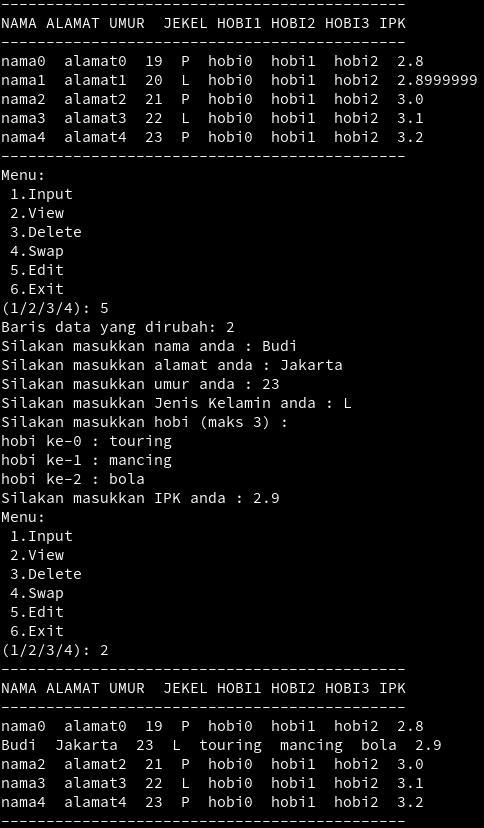
\includegraphics[scale=.7]{tug.png} 
\end{center}

\newpage

\section{Kesimpulan}
Setelah praktik mahasiswa dapat menambah data baru ke dalam larik dan dapat menghapus data tertentu dari dalam larik.

\end{document}
